%----------------------------------------------------------------------
\myframe{NASLib: A Modular and Extendable NAS Library \litw{Zela et al., 2020}}{

	\myit{
		\item Recap: Comparing head-to-head different NAS methods is difficult due to:
		\medskip
		\myit{
			\item[-] Different codebases
			\item[-] Different search and evaluation pipelines
			\item[-] Other confounding factors, e.g. library version, etc.
		}
		\pause
		\smallskip
		\item The main purpose of \textbf{NASLib} is to circumvent these issues by:
		\myit{
			\item[-] Providing a common language to implement all NAS methods and search spaces
			\item[-] Modularizing different components of NAS optimizers, e.g. one can go from DARTS to GDAS by just a method call
			\item[-] Offering the practitioner the opportunity to easily prototype new NAS methods
		}
		}

}
%----------------------------------------------------------------------

%----------------------------------------------------------------------
\myframe{NASLib: Overview}{
	\centering
	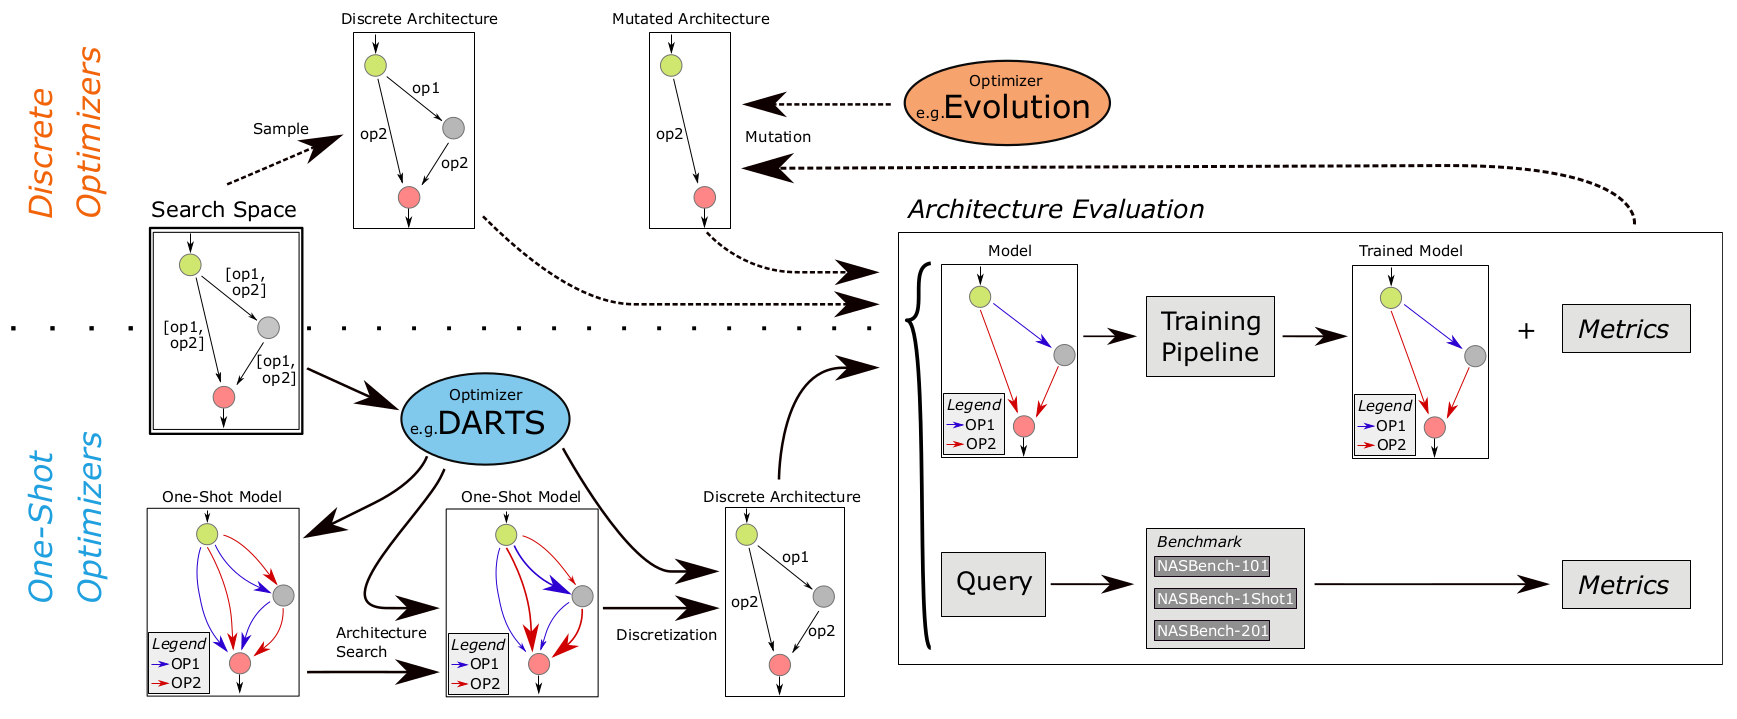
\includegraphics[width=0.85\textwidth]{images/naslib.png}\\
	
}
%----------------------------------------------------------------------

%----------------------------------------------------------------------
\myframe{NASLib building blocks: Search Spaces}{
	\centering
	TODO
	
}
%----------------------------------------------------------------------
%----------------------------------------------------------------------
\myframe{NASLib building blocks: Optimizers}{
	\centering
	TODO
	
}
%----------------------------------------------------------------------
%----------------------------------------------------------------------
\myframe{NASLib building blocks: Evaluators}{
	\centering
	TODO
	
}
%----------------------------------------------------------------------
%----------------------------------------------------------------------
\myframe{Tabular benchmarks for one-shot NAS}{
	\centering
	\myit{
		\item NAS-Bench-101 \lit{\href{https://arxiv.org/abs/1902.09635}{Ying et al. 2019}} does not support one-shot NAS methods due to its graph representation
		\medskip
		\pause
		\item \alert{NAS-Bench-1Shot1} \lit{\href{https://openreview.net/forum?id=SJx9ngStPH}{Zela et al. 2020}}
		\myit{
				\item[-] Maps the graphs in NAS-Bench-101 to a representations suitable for one-shot NAS methods
				\item[-] Based on some constraints it provides 3 sub-spaces of the original NAS-Bench-101 space
				\item[-] Currently the largest one-shot NAS tabular benchmark
			}
		\smallskip
		\pause
		\item \alert{NAS-Bench-201} \lit{\href{https://openreview.net/forum?id=HJxyZkBKDr}{Dong and Yang. 2020}}
		\myit{
				\item[-] Exact same graph representation as in DARTS
				\item[-] Much smaller than NAS-Bench-101 and NAS-Bench-1Shot1
				\item[-] Every architecture in the search space evaluated on 3 image classification datasets
			}
		}
}
%----------------------------------------------------------------------
%----------------------------------------------------------------------
\myframe{NASLib case study: Results on NAS-Bench-201}{
	\centering
	\begin{minipage}{.4\textwidth}
		\myit{
			\item<1-> NAS-Bench-201 is already integrated in NASLib and we can run any one-shot optimizer on that.
			\item<2-> Or apply random perturbations to every other one-shot optimizer.
			\item<3-> Also black-box optimizers can be evaluated cheaply with a tabular benchmark.
		}	
	\end{minipage}
	\begin{minipage}{.58\textwidth}
		\centering
		\visible<1->{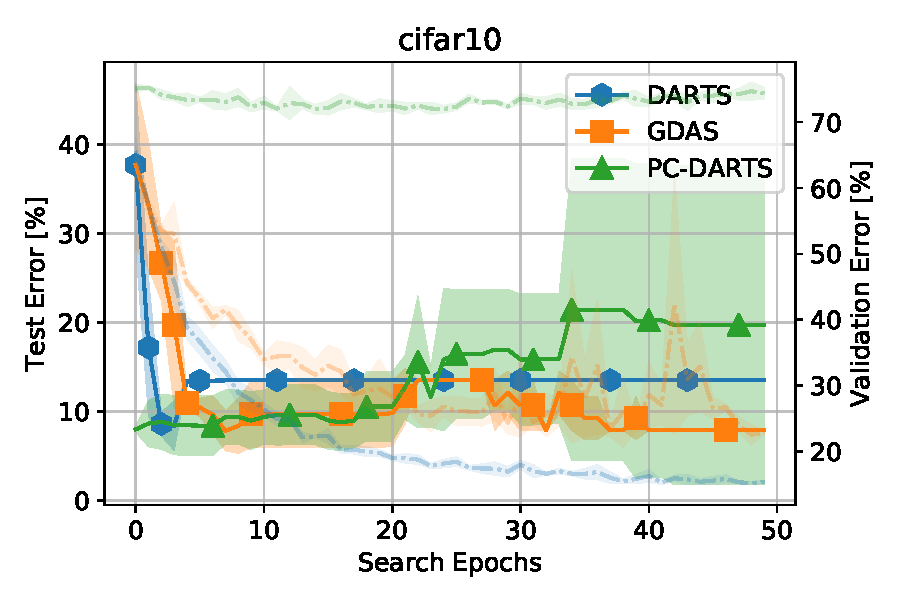
\includegraphics[width=0.45\textwidth]{images/nb201_1.pdf}}
		\visible<2->{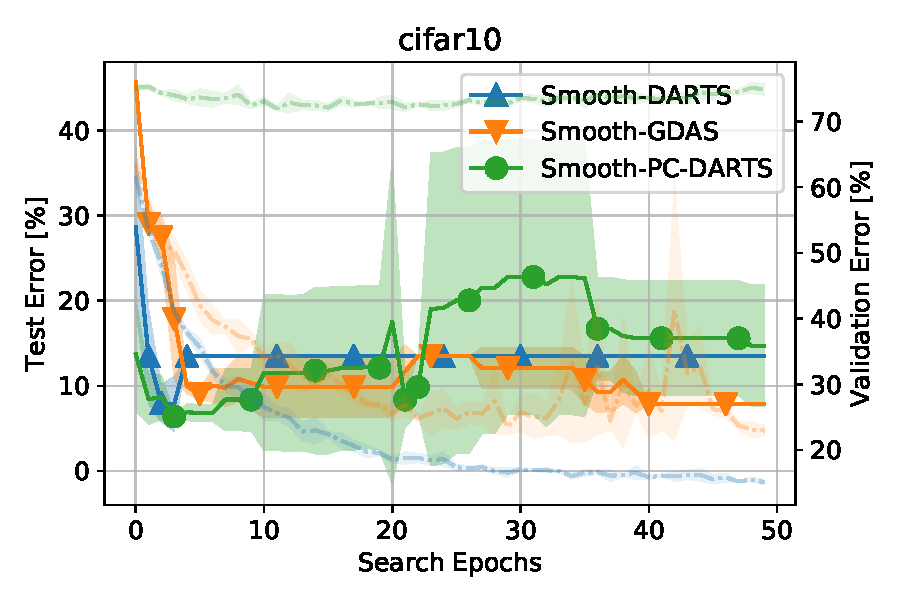
\includegraphics[width=0.45\textwidth]{images/nb201_2.pdf}}\\
		\visible<3->{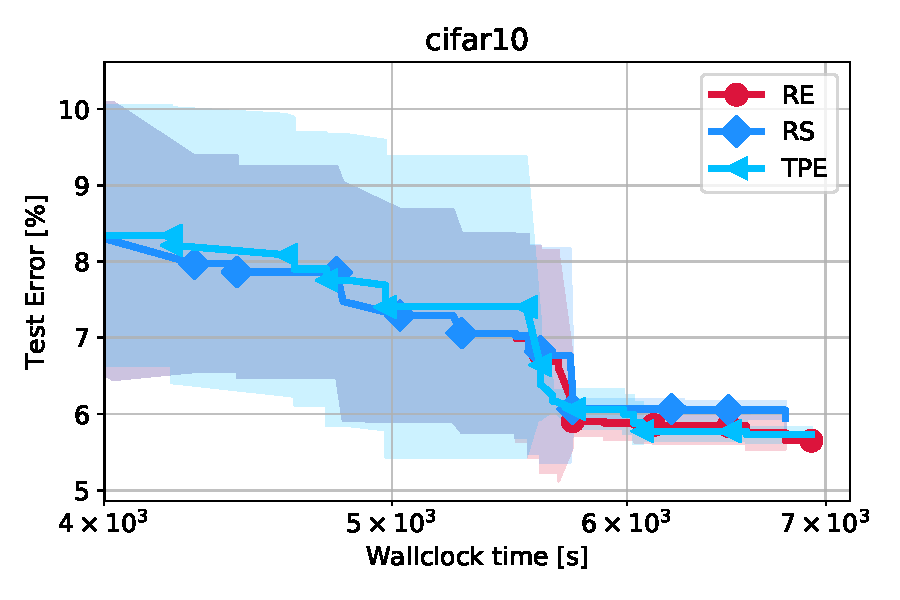
\includegraphics[width=0.55\textwidth]{images/nb201_3.pdf}}
	\end{minipage}
	
}
%----------------------------------------------------------------------



